\graphicspath{ {SectionTheRoadModule/Images/} }


\section{The Road Module}
\label{sec:the_road_module}



\subsection{Introduction}

The first step when using the SML World, is to set up the environment to be simulated. This environment consists in the definition of the roads where the cars can move, and how the environment looks (forest areas, dirt areas, river areas, etc...).

In this document two different things will be explained, in section \ref{sec:theroadnetwork} the construction and definition of the environment is explained. Section \ref{sec:roadmodule} explains how this environment can be used/interfaced with in the SML World.


\subsection{The Road Network}
\label{sec:theroadnetwork}

The road network determines the road setup and how can cars move in it. The road network definition is based on the ideas implemented in OpenStreetMap \cite{OSM}. The goal of the OpenStreetMap project is to provide a free geographic data, and allow users to contribute for the improvement of said maps.

\subsubsection{A quick introduction to OpenStreetMap}

The information here given is mostly taken from the OpenStreetMap Wiki page, more detailed information can be found there.

OpenStreetMap is based on three fundamental elements, nodes, ways and relations.

\begin{description}
  \item[Nodes] A node is an individual point on a map. Associated to each point is a set of GPS coordinates, latitude and longitude, and a unique indentifier, an id. Two or more nodes can be connected together to form complex shapes. This is done making use of ways. Figure \ref{fig:osm_nodes} shows a group of nodes.
  \item[Ways] A way is a line of nodes. This line is formed by connecting the nodes belonging to the way through straight segments. Several different ways can be formed with the same set of nodes, the order of the nodes in the way is then essential for it's correct definition. Ways can close on themselves, forming closed ways. Closed ways can be useful to define areas or regions. Figure \ref{fig:osm_way} shows an example of a way, notice that the way has a defined direction, if the nodes were ordered in reverse, the direction would be the opposite.
  \item[Relations]A relation is used to described more complex concepts that might involve multiple ways. That said a relation can be thought of as a grouping of ways, just like a way is a grouping of nodes. A relation is composed by it's members, and their roles in the relation.
\end{description}

\begin{figure}[h!]
  \centering
    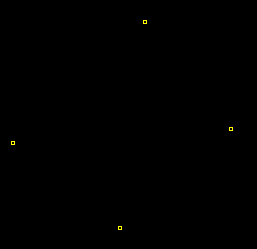
\includegraphics[width=0.5\textwidth]{osm_nodes}
    \caption{Visualisation of four nodes (visualisation using JOSM) \label{fig:osm_nodes} }
\end{figure}

\begin{figure}[h!]
    \centering
    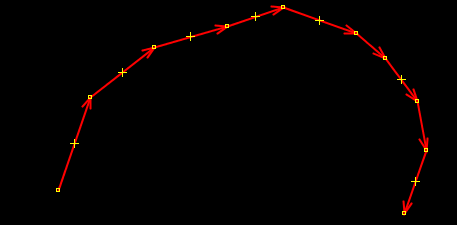
\includegraphics[width=0.5\textwidth]{osm_way}
    \caption{Visualisation of a way made up of ten nodes (visualisation using JOSM) \label{fig:osm_way} }
\end{figure}

Furthermore each of these elements can have tags. A tag is simply extra information that can be added to every element. A tag is defined by its name and value.

Making use of the simple concepts explained previously it is possible to define very complex maps.

\subsubsection{Adapting OpenStreetMap to the SML World}

In order to define our SML World road network, we will make use of the OpenStreetMap elements, however some additional concepts/conventions have to be defined.

\paragraph{Introduction to Lanelets}

Lanelets are the main concept used when defining the SML World road network. A lanelet is a particular case of an OSM Relation and it defines a road lane. Any road lane is defined by its limits (left and right lane markings). Road lanes also need a direction to be defined (unless they are bi-directional).

The creation of a lanelet is as follows:

\begin{enumerate}
\item Create the way (and respective nodes) corresponding to the left lane markings
\item Create the way (and respective nodes) corresponding to the right lane markings
\item Create a relation, and add as members the previous ways, with the respective roles, left\_lane\_marking and right\_lane\_marking
\end{enumerate}

The direction of the lanelet is defined by the direction of the right\_lane\_marking way. Whatever the direction of left\_lane\_marking might be, the direction of the lanelet will be the same as the direction of the right\_lane\_marking way.

Let us imagine we wish to define the road shown in figure \ref{fig:road_to_define}. These road is section is composed of two lanes, and as such we will need two lanelets to define this road. First we need to define the ways, that correspond to the left and right lane markings. In order to create these ways, we need first to add the corresponding nodes. Figure \ref{fig:road_to_define_with_nodes} shows the nodes that need to be created in order to define the ways corresponding to the lane markings. Once these nodes are added, we simple create the respective ways, as shown in figure \ref{fig:road_to_define_with_ways}. The orange and pink ways, will be the right\_lane\_marking of each lanelet, whilst the blue way will be the left\_lane\_marking of both lanelets. Note that the direction of the right lane marking will always define the direction of the lanelet, and as such it is important that this way is correctly oriented. It might be confusing that the same way, and the same direction, is used for the left\_lane\_marking of both lanelets, but this will not be a problem, as we simply use the left\_lane\_marking of a lanelet to know where a lane boundary is, not its direction.

\begin{figure}[h!]
  \centering
    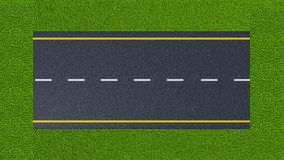
\includegraphics[width=0.5\textwidth]{road_original}
    \caption{The road section that we wish to define \label{fig:road_to_define} }
\end{figure}

\begin{figure}[h!]
    \centering
    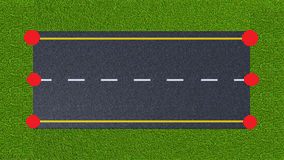
\includegraphics[width=0.5\textwidth]{road_with_nodes}
    \caption{Road section overlayed with necessary nodes \label{fig:road_to_define_with_nodes} }
\end{figure}

\begin{figure}[h!]
    \centering
    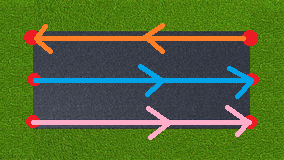
\includegraphics[width=0.5\textwidth]{road_with_ways}
    \caption{Road section overlayed with necessary ways \label{fig:road_to_define_with_ways} }
\end{figure}

\paragraph{Defining a Road Network using Lanelets}

A road network can be created making use of several lanelets. First however we need to define the concept of Lanelet Adjacency.

\textbf{Lanelet Adjacency} Two lanelets, $L_a$ and $L_b$, are said to be adjacent if the first node of the right\_lane\_marking of $L_b$ is the same as the last node of the right\_lane\_marking of $L_a$.

When two lanelets are adjacent, we know that a car can travel from one lanelet to the other. The importance of the lanelet adjacency stems from the need of needing to generate realistic and law-conforming paths for the cars to drive on.

Figure \ref{fig:intersection_original} shows a three way intersection with the corresponding lanelets that lead into it. The lanelets are shown in a very simplified way, by a straigh segment in the middle of each lanelet. With each segment there is an associated arrow, indicating the direction of the lanelet.

\begin{figure}[h!]
    \centering
    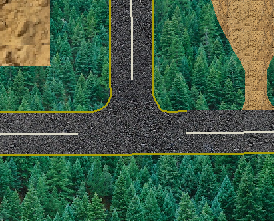
\includegraphics[width=0.5\textwidth]{intersection_original}
    \caption{A three way road intersection \label{fig:intersection_original} }
\end{figure}

The lanelets that describe the possible movements in this intersection are shown in figures \ref{fig:intersection_paths_group_1}, \ref{fig:intersection_paths_group_2} and \ref{fig:intersection_paths_group_3}.

\begin{figure}
    \centering
    \begin{subfigure}[b]{0.3\textwidth}
        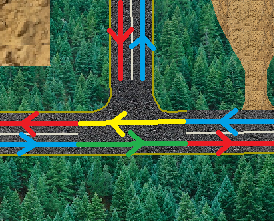
\includegraphics[width=\textwidth]{intersection_paths_group_1}
        \caption{Lanelets connecting left and right sections}
        \label{fig:intersection_paths_group_1}
    \end{subfigure}
    ~ %add desired spacing between images, e. g. ~, \quad, \qquad, \hfill etc. 
      %(or a blank line to force the subfigure onto a new line)
    \begin{subfigure}[b]{0.3\textwidth}
        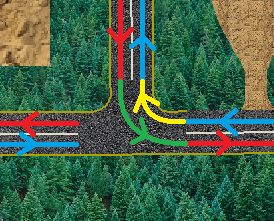
\includegraphics[width=\textwidth]{intersection_paths_group_2}
        \caption{Lanelets connecting top and right sections}
        \label{fig:intersection_paths_group_2}
    \end{subfigure}
    ~ %add desired spacing between images, e. g. ~, \quad, \qquad, \hfill etc. 
    %(or a blank line to force the subfigure onto a new line)
    \begin{subfigure}[b]{0.3\textwidth}
        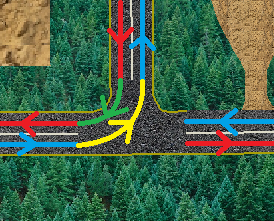
\includegraphics[width=\textwidth]{intersection_paths_group_3}
        \caption{Lanelets connecting top and left sections}
        \label{fig:intersection_paths_group_3}
    \end{subfigure}
    \caption{All the possible lanelets in a three way intersection}
\end{figure}

When all the lanelets of the intersection are put together, we create a functional piece of road network, with well defined car paths. Remember that a car can only travel between adjacent lanelets, and as such the road intersection does not allow for illegal movements, such as moving to a lane with a different direction.

Using this concept of lanelets and lanelet adjacency we can create a big variety of road networks with well defined rules of traffic flow. This is of extreme importance as we will see in the following sections.

MAYBE DO A LIST OF ADJACENCIES.

\subsubsection{Creating a Road Network}

Once the concepts of the road network are understood, we can start creating one. For this purpose we will use JOSM.

\paragraph{JOSM}

JOSM\cite{JOSM} is an OpenStreetMap editor. This editor provides a GUI to edit OpenStreetMap files/maps. We will make use of it to create a file that will define our road network. Figure \ref{fig:josm_sml} shows a snapshot of a JOSM program instance running.

\begin{figure}[h!]
    \centering
    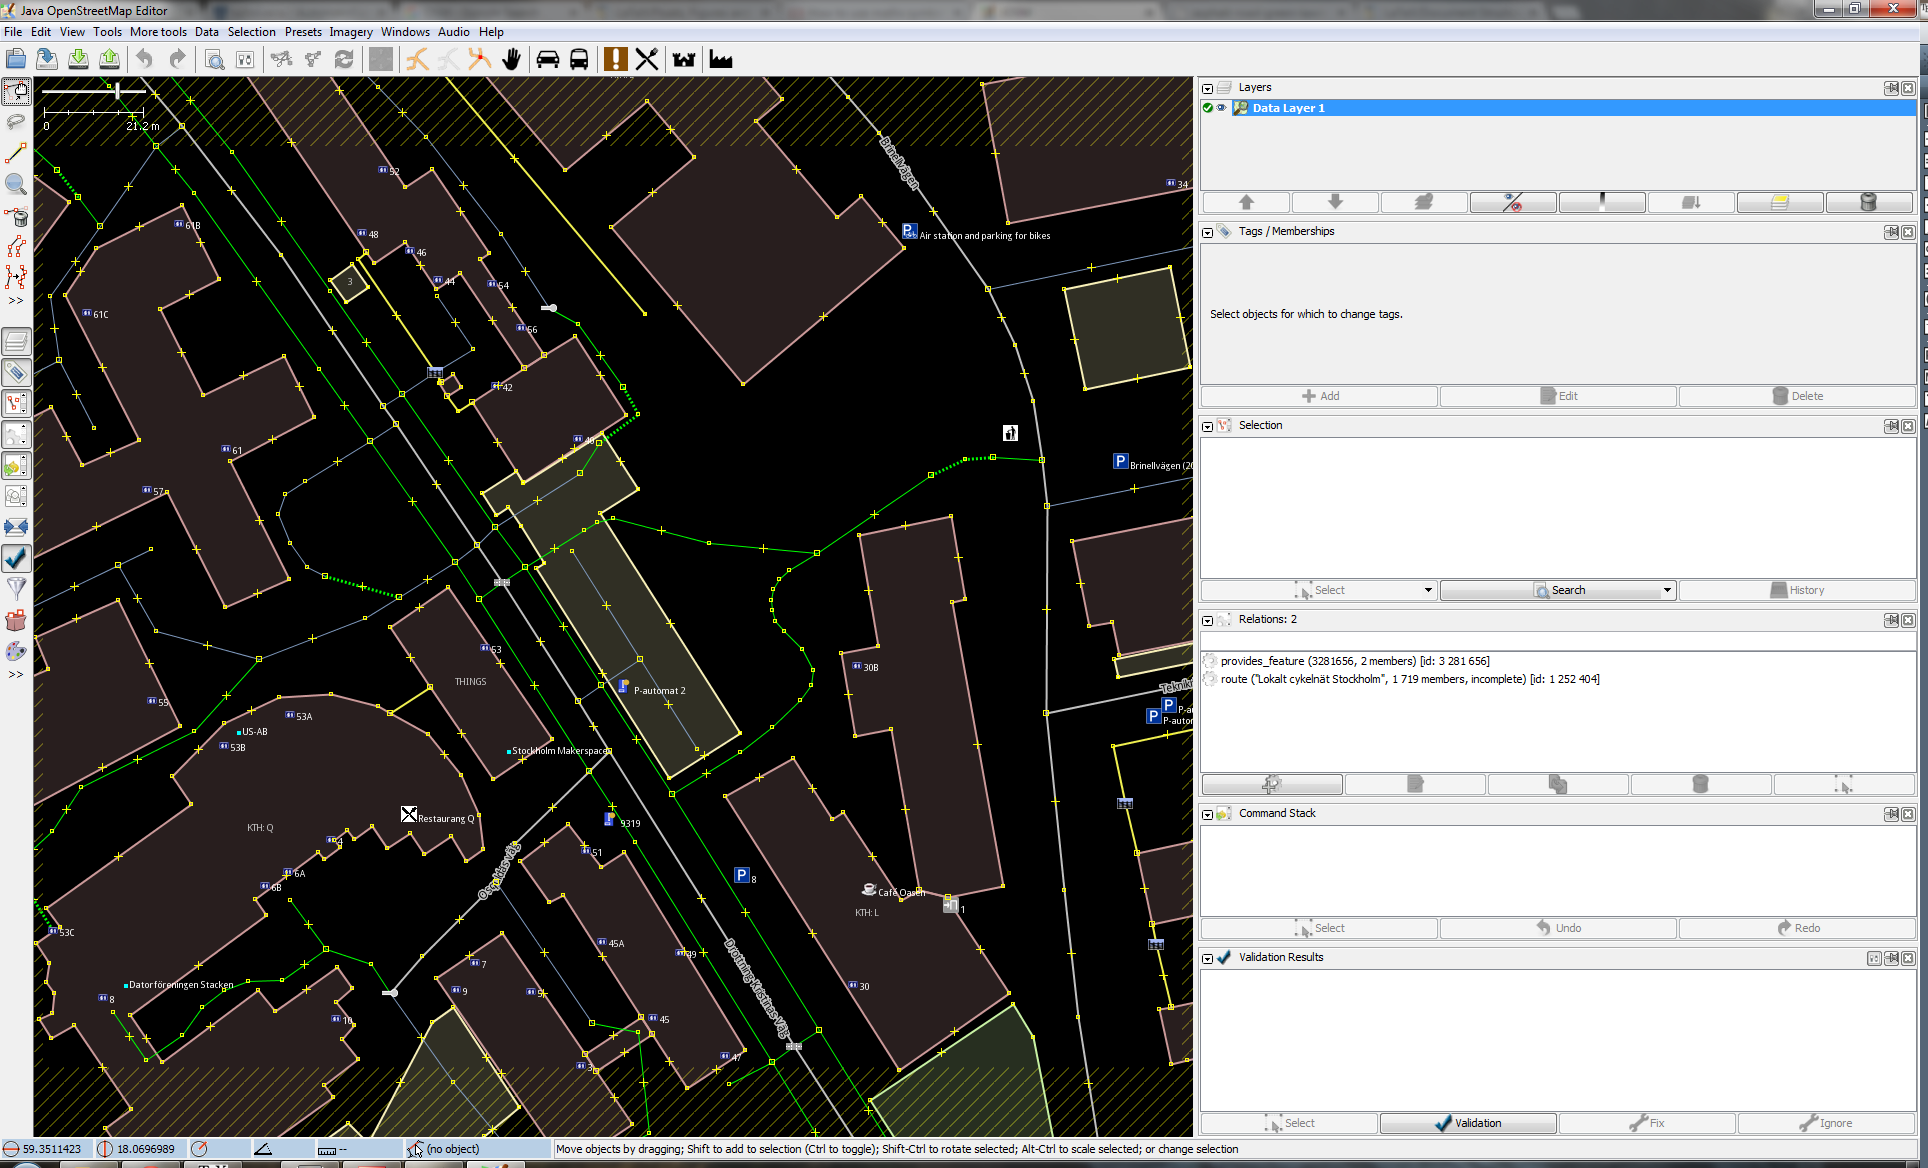
\includegraphics[width=0.75\textwidth]{JOSM_SML}
    \caption{An overview of the SML and surroudings OpenStreetMap map making use of JOSM \label{fig:josm_sml} }
\end{figure}

Here it will not be explained how to use JOSM, only how to build our road network making use of it. To understand how to work with JOSM refer to the guide available online.

\paragraph{Creating a Lanelet}

Before creating a lanelet, we need to create the ways corresponding to its left and right road markings. Lets start by creating the right road marking. To do so we simply create a way with the orientation that we wish our lanelet to have.

We could now use the same procedure to create the left road marking, however we are going to make use of the parallel tool to remove the ammount of work that placing the nodes requires. Besides being more efficient the parallel tool also guarantes that the new lane marking is parallel and in the same shape as the original lane marking, which should happen in every road.

An important detail is that the lanelet road marking ways need to have the same ammount of nodes, otherwise they cannot be processed by the SML World. The parallel tool complies with this requirement.

Once both ways are defined, we simply need to create our relation, which will represent a lanelet. Simply create a new relation, and the tag "type"="lanelet" and associate as members "right\_road\_marking" and "left\_road\_marking" the respective ways. The lanelet is now defined. 

\paragraph{Connecting Lanelets}

To connect lanelets, i.e., to make them adjacent we simply need to make sure that they have the same orientation, and that the first node of right way in one of the lanelets corresponds to the last node in the other lanelet.


\paragraph{Saving the Road Network File}

When the road network is complete, its corresponding information must be saved. JOSM allows saving the road network in several different file types, however we are interested in saving the file with the \textit{.xml} extension, meaning that we will have a simple to read XML file that can be easily used for future purposes.

If we wish to edit a previously save map, we simply need to open the corresponding \textit{.xml} file, edit it and save it again.

\paragraph{General Tips}

Using the parallel tool is often a good practice, due to the reasons already stated.

JOSM provides several tool, however that are some extra tools that can be added through the use of plugins. One of these tools is Circle Arc, which allows the user to draw circle arcs with relative ease.


\paragraph{List of Existing Road Networks OSM Files}

Some Road Networks were already made for previous usages. Their filenames and an explanation of their purposes will be given here.

\begin{description}

\item[HighwaySML.xml] This is the road network of a circular Highway with three lanes, all in the counter clockwise direction. This road network was used by the Summer Students of 2015, and it served to show possible solutions to the GCDC scenarios of platoons merging and emergency vehicle. The highway dimensions were fitted so that they allow for real live demonstrations using the scaled trucks. This road network can be altered to larger dimensions for simulation purposes.
\item[MiningEnvironmentSML.xml] This defined the road network used in the May 2015 IQMatic demonstration at Scania. It is composed of several roads and intersections, and it special environments for the scaled trucks to perform Autonomous Driving manoeuvres, like reverse driving and path planning. This map is not supported by the current SML World version, but can be useful in the creation process of new maps.
\item[SodertaljeResidentialArea.xml] This road network was based on a real residential road network. Defining road networks based on real existing ones can be useful to show and evaluate the performance of the autonomous driving system in realistic scenarios. This map is not supported by the current SML World version.
\item[RoadTemplates.xml] This file contains some useful and complex road network elements, like three and four way intersections. They can be easily copied for the creation of new maps.
\end{description}




\subsection{The Road Module}
\label{sec:roadmodule}

The Road Module is the name given to the Python class present in the SML World that is responsible for all the functionalities related to the road network. Its functionalities can be divided into two broad scopes, the computation of car trajectories and the visualisation of the environment.

In this section, we will give an overview of the functionalities that the Road Module provides, and an explanation of it's internal algorithms, when necessary.

\subsubsection{Processing the Road Network Map}

The first task of the Road Module, is to process and make sense of the Road Network Map. To do so, the constructor of the class is provided with the \textit{.xml} file containing this information.

The constructor will parse the \textit{.xml}, and the class will store dictionaries for the existing nodes, ways and lanelets in said file. Additionally a dictionary storing all the found tags, and corresponding nodes, is also created.

\paragraph{Converting from GPS to Meters}

As stated previously every OSM Node has an associated GPS latitude and longitude. For our purposes, we wish to have a simpler representation of the spatial location of the nodes, such as a Cartesian coordinate system in meters.

To do so we make use of the Python package \textbf{utm} (https://pypi.python.org/pypi/utm). This package allows us to make a conversion from GPS coordinates to a Cartesian referential as defined by the UTM convention. Once we have these new coordinates we will apply a translation transform so that they will be defined in a more convenient referential.

By default this new referential is located in the center of all the OSM Nodes. This center is computed easily by averaging the position of all the nodes. Once we know this center, we just need to subtract it from the coordinates of every single node, we will then have all of the node coordinates in the referential located in the center of all the nodes.

Another possibility is to define an Origin Node on which the referential will be located. To do so, when creating the \textit{.xml} file, one just need to and a node with the tag "origin"="true". If the Road Module detects that such a node is present in the file, it will simply subtract this node's Cartesian coordinates to all of the other nodes' coordinates, effectively making them be referenced on a referential located at the origin node.

\paragraph{Computing Lanelet Adjacencies}

One of the most important parts of the road network is the adjacency between the lanelets, for it defines the possible ways that cars can drive in them.

To fully describe the adjacencies between lanelets, we will make use of an Adjacency Matrix. An adjacency matrix A, is a square matrix with $n \times n$ elements, where $n$ is the number of lanelets in the road network.

\[
A_{n,n} = 
 \begin{pmatrix}
  a_{1,1} & a_{1,2} & \cdots & a_{1,n} \\
  a_{2,1} & a_{2,2} & \cdots & a_{2,n} \\
  \vdots  & \vdots  & \ddots & \vdots  \\
  a_{n,1} & a_{n,2} & \cdots & a_{n,n} 
 \end{pmatrix}
\]
 
The entry $a_{i,j}$ in the matrix indicates the adjacency value between lanelet $i$ and lanelet $j$. If its is possible to go from lanelet $i$ and lanelet $j$, \textit{i.e.}, if it lanelet $i$ is adjacent to lanelet $j$, the value of $a_{i,j}$ will be equal to the length of lanelet $i$.

If the it is not possible to go from lanelet $i$ and lanelet $j$, the value of $a_{i,j}$ will be infinity, or an extremely large number (in the SML World implementation this value is $10^{10}$).

Notice that $a_{i,j}$ is not necessarily equal to $a_{j,i}$, as being able to go from lanelet $i$ to lanelet $j$, does not imply that it is possible to go from lanelet $j$ to lanelet $i$.

\subsubsection{Computing Car Paths}

Computing a car path is equivalent to finding a valid/feasible way of going from one point in the road network to another. To do so, we divide this process in several parts.

\paragraph{The Start and End Nodes of the Path}

The main inputs to the Path Finding algorithm are the Start Node and the End Node. The start and the end nodes define, respectively, where we wish our path to start, and where we want it to end.

Given the start node, the Road Module will find the lanelet (or lanelets) that have this node in as part of their right\_lane\_marking way. For now lets assume that only one lanelet contains this node. The same is done for the end node, and the lanelet containing it is found. We now have two lanelets that we will call $lanelet_{start}$ and $lanelet_{end}$, which contain the start and end node, respectively.

We now have a way to move from $lanelet_{start}$ to $lanelet_{end}$. The solution to this problem will be a path of lanelets, that will start in $lanelet_{start}$ and finish in $lanelet_{end}$, making only legal movements, \textit{i.e.}, transitions between adjacent lanelets.

\paragraph{The Dijkstra Algorithm}

We wish to go from the starting lanelet to the ending lanelet, making transitions only between lanelets that are adjacent. We also want to do it in the best way possible, \textit{i.e.}, shortest way possible. 

This problem can be easily solved using the well known Dijkstra Algorithm. The Dijkstra algorithm is able to find the shortest path between nodes in a graph. We can view our road network as a graph of lanelets, in fact, the Lanelet Adjacency Matrix, perfectly defines a graph, where the lanelets are the nodes of the graph, and the edges are defined by the weights given by the adjacency matrix elements. An element of the matrix with an infinite value is equivalent to a non-existing edge.

This means, that having $lanelet_{start}$, $lanelet_{end}$, and the lanelet adjacency matrix, we can run the Dijkstra algorithm, and find the shortest path of lanelets between $lanelet_{start}$ and $lanelet_{end}$.

\paragraph{Generating the Path}

Assume now, that after our Dijkstra algorithm, we found a solution path $ [lanelet_{start},\allowbreak lanelet_{a},\allowbreak lanelet_{b},\allowbreak lanelet_{c},\allowbreak lanelet_{end}]$. We now wish to get the $(x,y)$ path corresponding to this lanelet path. 

The $(x,y)$ path of a lanelet, which is the set of points centred between the left\_lane\_marking and right\_lane\_marking, where each point is equally distant to the next and previous points.

We compute the $(x,y)$ path for each lanelet in the lanelet path, stitch them together, forming an $(x,y)$ from $lanelet_{start}$ to $lanelet_{end}$ that complies with the rules of the road network (as defined in the lanelet adjacency matrix).

This path still needs a final modification, however. The path is made up of the full $(x,y)$ paths of each lanelet, including the $lanelet_{start}$ and $lanelet_{end}$, however we might not need the full path of the $lanelet_{start}$ and $lanelet_{end}$. Take for example the case where the prvided ending node is located somewhere in the middle of $lanelet_{end}$. In this case we will not want the full $(x,y)$ path of the lanelet, but only the section that starts at the beginning of the lanelet, and ends close to he ending node. The same principle applies to the $(x,y)$ path of $lanelet_{start}$, however resulting path will begin at the starting node and continue until the end of the lanelet. We call this procedure, cropping the trajectory.

\paragraph{The "Circular" Dijkstra Algorithm}

The "Circular" Dijkstra algorithm is a special situation of the Dijkstra algorithm, in which we wish to find the shortest way from a node to itself, whilst assuming that nodes cannot connect to themselves. The importance of this algorithm for the SML World, has to do with generating paths that loop, thus resulting in motions that can run forever.

The original previous formulation of the Dijkstra algorithm does not allow us to solve this problem, however a simple reformulation can be done, that will allow us to find the shortest path from a node to itself.

To solve this problem we will need to create a new graph, that will be equivalent to the original graph, but that will allow us to solve the problem. Given that we want to find the shortest path from $node_i$ to itself, we will have to replace $node_i$ by nodes $node_i^{start}$ and $node_i^{end}$. $node_i^{start}$ will have all of the outgoing edges of $node_i$, and $node_i^{end}$ will have an of the incoming edges of $node_i$. 

Once this new graph is defined we can simply run a Dijkstra algorithm to find the shortest path between $node_i^{start}$ and $node_i^{end}$, and this will be equivalent to the shortest path from $node_i$ to itself.

\subsubsection{Environment Visualisation}

Besides defining how the road network behaves, the Road Module is also responsible for how the environment looks like. This is an important task as the visualisation of the environment plays a big role in the SML World.

Generating and visualising the environment requires the use of the graphical library pygame. More information about pygame can be found in their website \cite{pygame}.

\paragraph{Drawing Patterns}

The first step consists in generating the environment background. For this purpose we start by repeating the pattern image that we wish to fill the background with. Usually we use a forest pattern as can be seen in figure \ref{fig:visualisation_background}. The forest pattern is simply applied through the whole image, as it is a background pattern. One can choose different any possible background by selecting the appropriate image pattern.

\begin{figure}[h!]
  \centering
    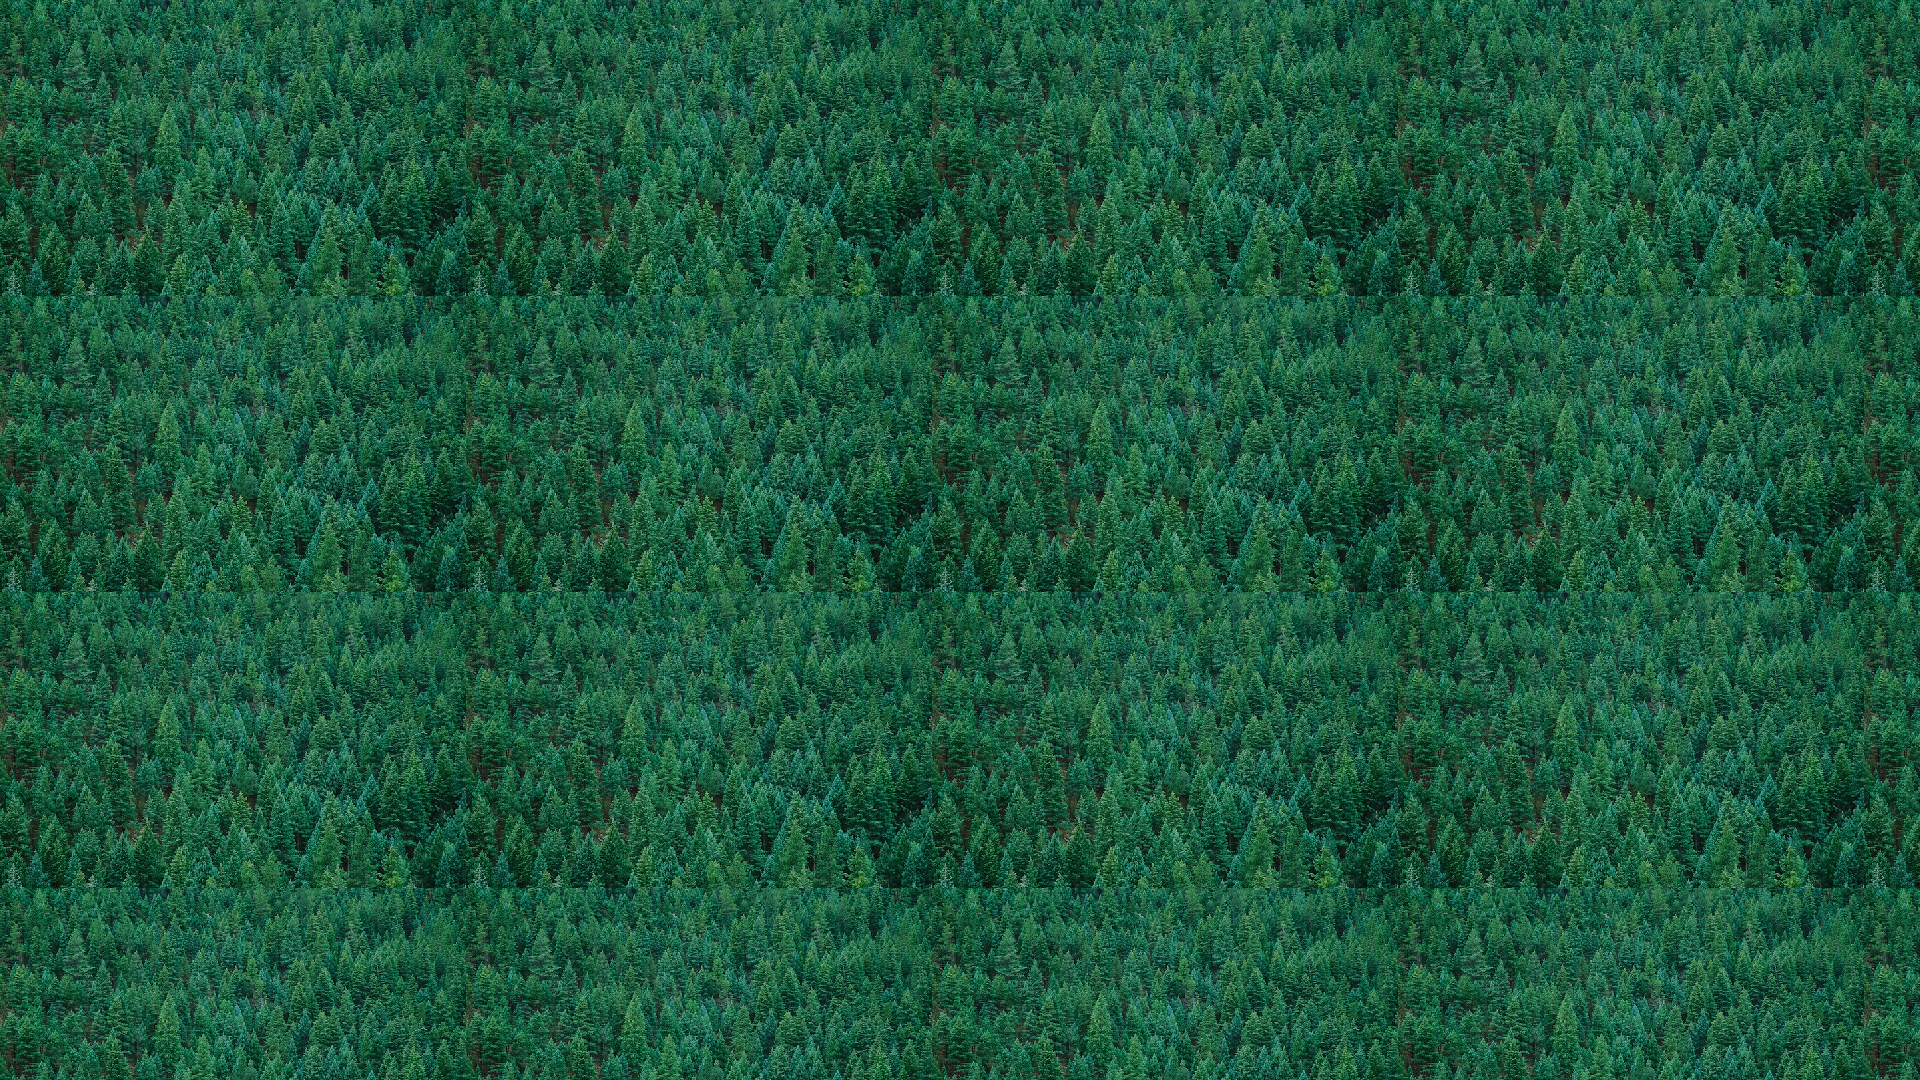
\includegraphics[width=0.95\textwidth]{visualisation_background}
    \caption{An environment with a forest pattern as background \label{fig:visualisation_background} }
\end{figure}

Once the background is drawn, we will overlay it with the roads. The roads are simply drawn by repeating a road pattern in the pixels corresponding to lanelets. First we find the regions of the lanelets, also called a mask. This mask tells us all the pixels that correspond to lanelets. Once we know this mask, we know where the lanelets are. We use this information to repeat the road pattern in the regions where there are lanelets. The result is shown in figure \ref{fig:visualisation_background_and_roads}. We can choose different looks for the roads by simply selecting the appropriate pattern image. 

\begin{figure}[h!]
  \centering
    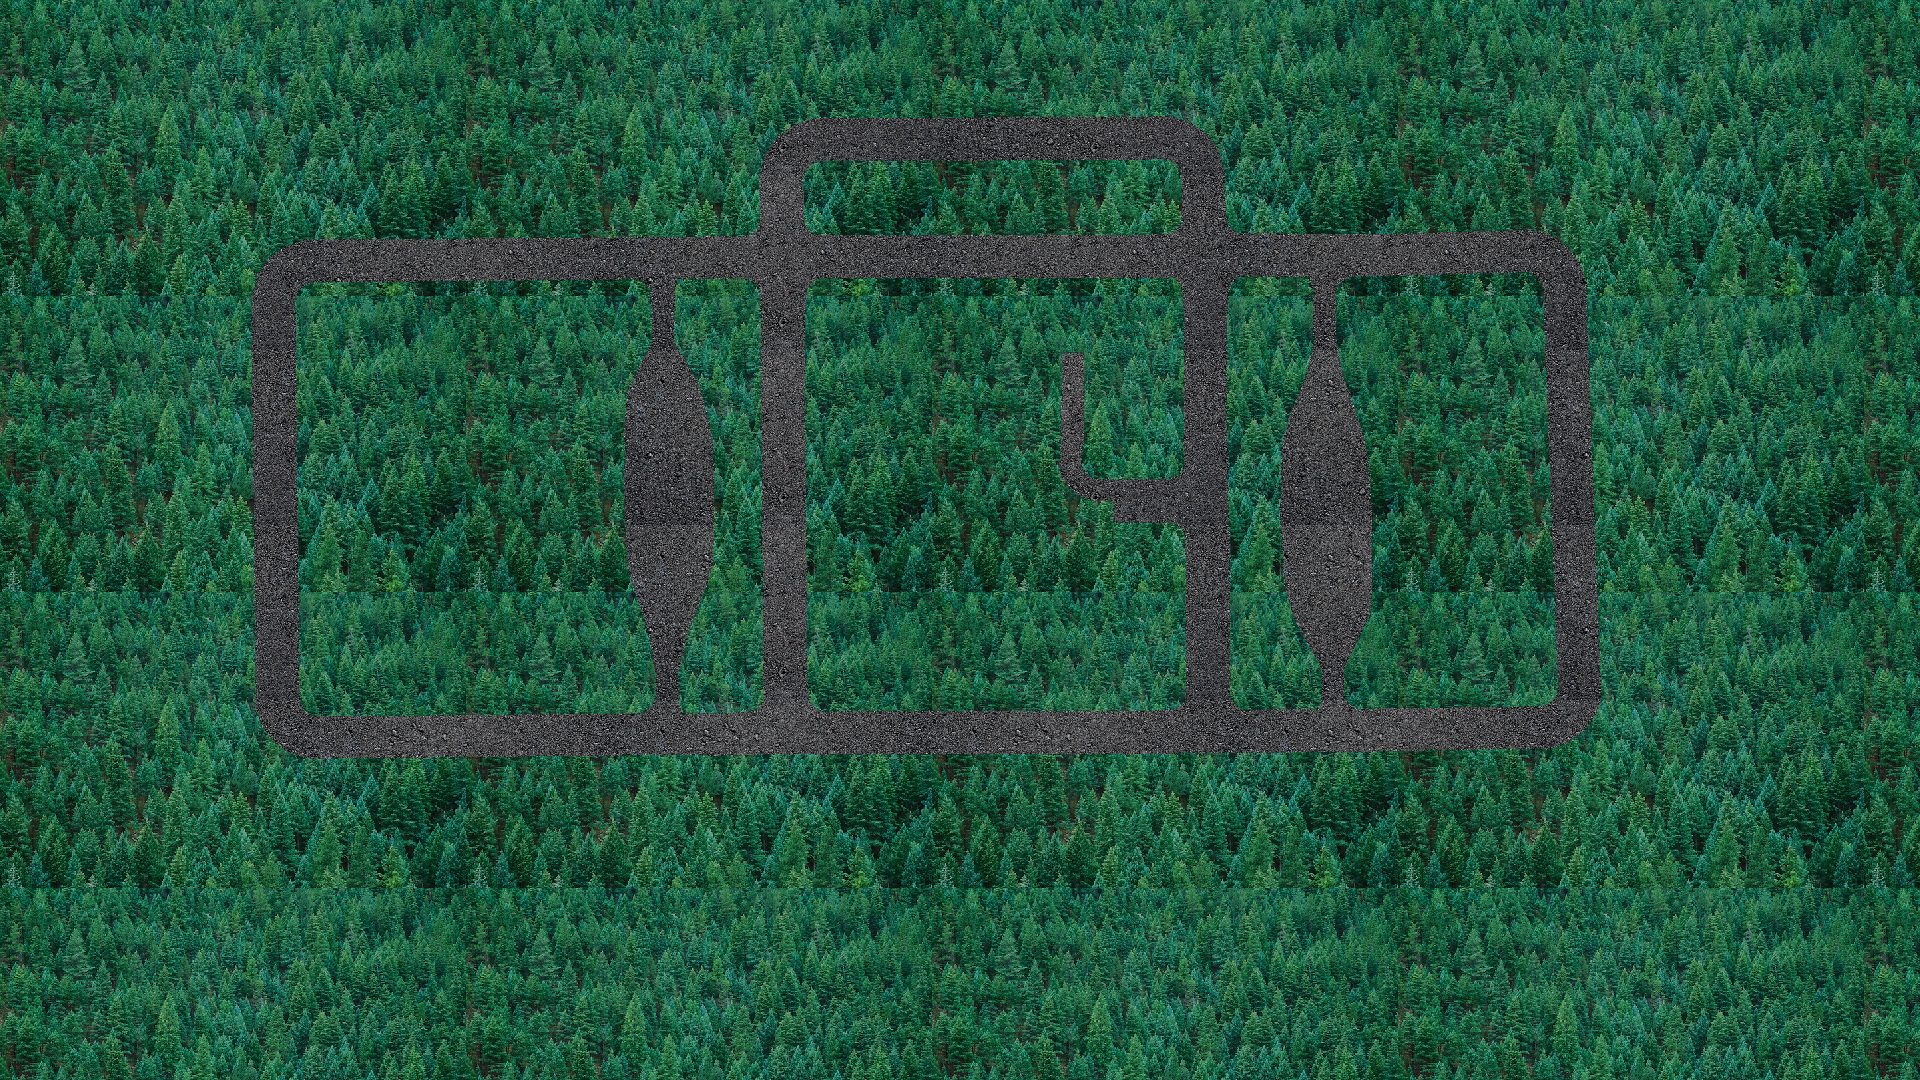
\includegraphics[width=0.95\textwidth]{visualisation_background_and_roads}
    \caption{An environment with a road pattern added \label{fig:visualisation_background_and_roads} }
\end{figure}

The environment visualisation can be made arbitrarily complex, if one uses this pattern repeat functionality to draw several different regions of different types. Figure \ref{fig:visualisation_background_with_several_patterns} shows an environment using five different patterns: forest, road, mud, iron and parking lot.

\begin{figure}[h!]
  \centering
    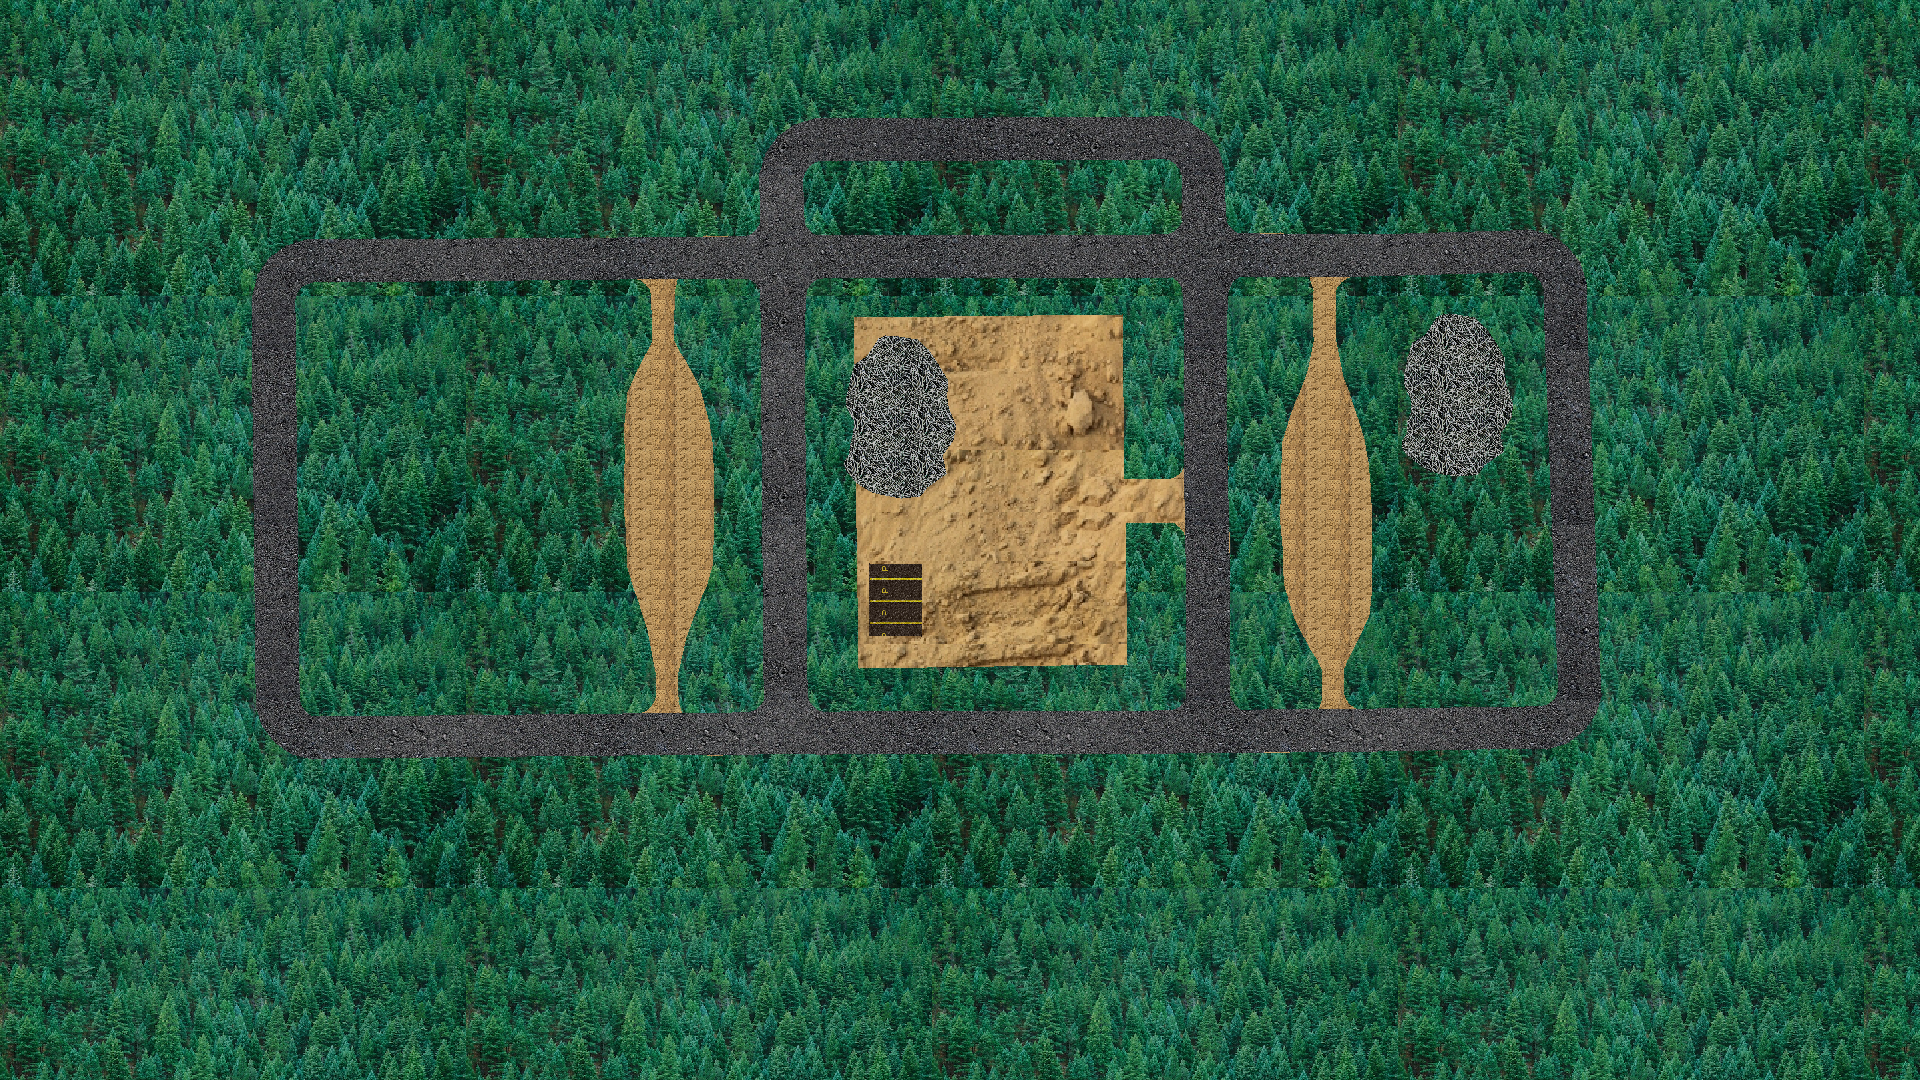
\includegraphics[width=0.95\textwidth]{visualisation_background_with_several_patterns}
    \caption{An environment using several patterns \label{fig:visualisation_background_with_several_patterns} }
\end{figure}

\paragraph{Drawing Lines}

Another important part of the environment visualisation is the ability to draw lines. Drawing lines comes in handy when drawing road markings. The road module is able to draw lines of different colors and different widths for ways that are present in the road network, this can be seen in figure \ref{fig:visualisation_background_and_roads_and_markings}. The road module will go over all of the ways present in the road network and it will draw lines on top of them if they have a specific tag. In case they have a tag "line\_type"="interior", they will be drawn as a white line, if the tag is "line\_type"="exterior" they will be drawn as yellow lines. If a way has no tag, a line is not drawn. 

\begin{figure}[h!]
  \centering
    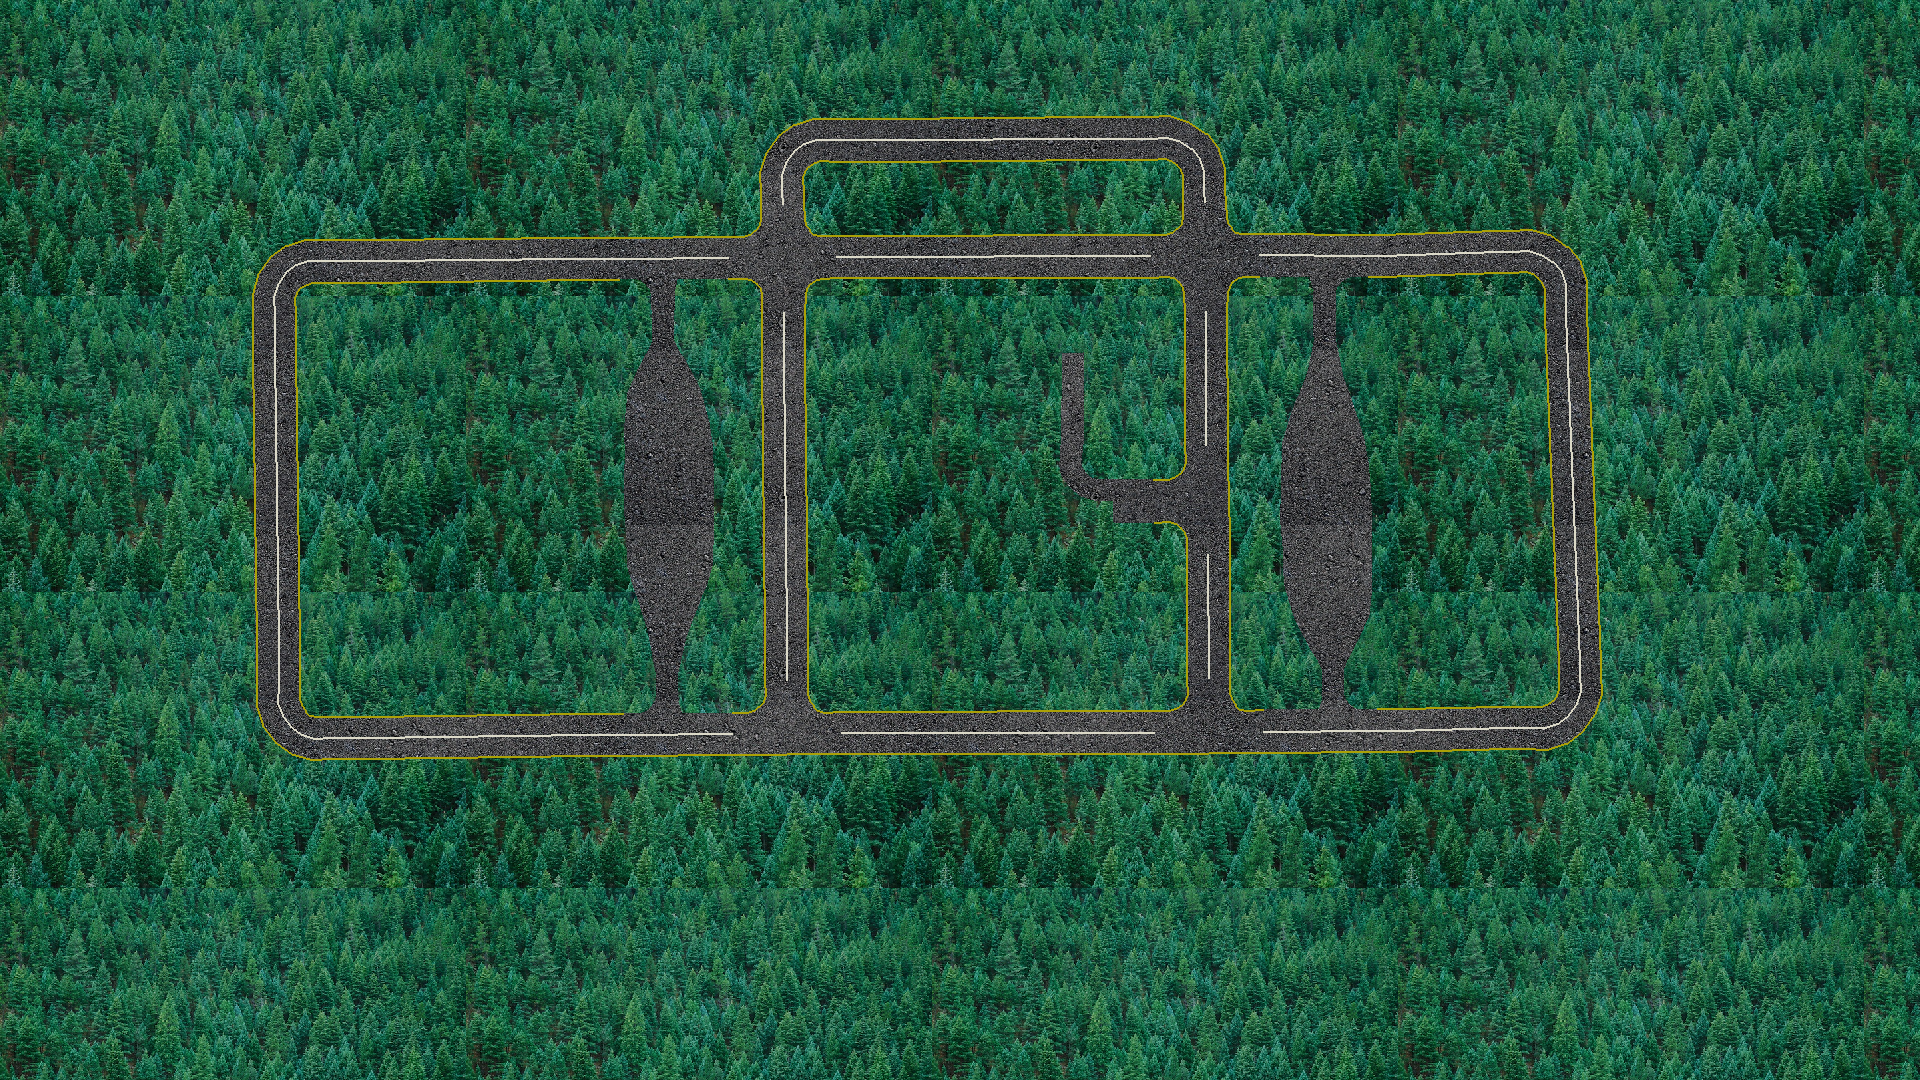
\includegraphics[width=0.95\textwidth]{visualisation_background_and_roads_and_markings}
    \caption{An environment with lines drawn \label{fig:visualisation_background_and_roads_and_markings} }
\end{figure}

\subsubsection{Using the Road Module}

Here we will briefly explain the main usages of the Road Module from a programming point of view. More detailed information is available in the source code.


\paragraph{RoadModule()}

road\_module = RoadModule(xml\_file\_location) Constructs an instance of the class \texttt{RoadModule}. The constructor requires that the location of the \textit{.xml} defining the road network is given.

\paragraph{SetImageProperties()}

SetImageProperties sets the properties of the image that will correspond to the environment. As arguments ImageWidth and ImageHeight correspond to the desired image width and height in pixels. PixelPerMeter will define how many pixels correspond to a meter in the map. Decreasing the value of PixelPerMeter will make the image correspond to a larger environment area.

\paragraph{GetEnvironmentImage()}

GetEnvironmentImage generates and returns the image of the enviroment. The arguments required are the same as the ones in SetImageProperties. This method returns a pygame Surface corresponding to the environment image.

\paragraph{GetPathBetweenNodeIds()}

GetPathBetweenNodeIds returns an $(x,y)$ path between two nodes. The arguments are StartOsmNodeId and EndOsmNodeId, which correspond to the ids of the nodes we wish that define this path. The third argument is PointsPerMeter wich indicates how many path points will be generated for each meter of path.

\paragraph{GetPathBetweenNodeTags()}

Equivalent to GetPathBetweenNodeIds, however instead of having node ids as arguments, we have node tags. This allows for a simpler usage, as it is usually easier to know the tag of a node (it can be easily added on the road network \textit{.xml} file), than its id.

\paragraph{GetClosedPathFromNodeId()}

Returns the $(x,y)$ path that starting and ending on a given node. The arguments are OsmNodeId and PointsPerMeter. OsmNodeId corresponds to the id of the node we wish to have the circular path of. PointsPerMeter will define how many path points will be generated for each meter of path.

\paragraph{GetClosedPathFromNodeTag()}

Equivalent to GetClosedPathFromNodeId, however istead of providing a node id, the user provides a node tag.

\subsubsection{Deprecated Functionalities}




Talk about how to draw patterns given a way and a tag.

